\documentclass[aspectratio=1610]{beamer}
\usetheme{boxes}
\usecolortheme{crane}
\usepackage{amsmath,amsfonts}
\usepackage{algpseudocode}
\usepackage{multicol}
\usepackage{pgfplots}
\pgfplotsset{compat=1.15}
\usepackage{mathrsfs}
\usetikzlibrary{arrows}


%-------------------------------------------------------------------
%	 TITLE SLIDE
%-------------------------------------------------------------------


\begin{document}

% -------------------------------------------------------------------
% Lesson 2
% -------------------------------------------------------------------
\section{Software specifications. Formal methods}

\begin{frame}
\begin{center}
\Huge Lesson 2\\~\\
\textbf{Software specifications. Formal methods}
\end{center}
\end{frame}


\begin{frame}
\frametitle{Lesson 2}

\Huge In this lesson we will talk about:
 \alert{Software specifications},
 \alert{Formal methods},
 \alert{Software verification and validation}
\end{frame}



\begin{frame}
\begin{center}
\Huge
\begin{quote}
\textbf{"Todays software has grown by evolution, not by intelligent design"}
\begin{flushright}
{--- Leslie Lamport}	
\end{flushright}
\end{quote}
\end{center}
\end{frame}


\begin{frame}{Lesson 2}{}
\includegraphics[scale=0.30]{Images/loc.png}
\end{frame}


\begin{frame}{Lesson 2}{}
\Huge
 Our software is getting more and more \textbf{complex}, \textbf{buggy} and \textbf{difficult} to maintain.
 \end{frame}


\begin{frame}[plain,noframenumbering]
\makebox[\linewidth]{\includegraphics[width=\paperwidth]{Images/outage1}}
\end{frame}

\begin{frame}[plain,noframenumbering]
\makebox[\linewidth]{\includegraphics[width=\paperwidth]{Images/outage2}}
\end{frame}

\begin{frame}[plain,noframenumbering]
\makebox[\linewidth]{\includegraphics[width=\paperwidth]{Images/outage3}}
\end{frame}

\begin{frame}{Lesson 2}{}
\Huge
\center
    \textbf{What can we do about it?} 
\end{frame}



\begin{frame}{Lesson 2}{}
\Huge
\center
   Start with a \textbf{smart design} at the specification level
\end{frame}


\begin{frame}{Lesson 2}{}
\begin{center}
\Huge\textbf{Software Specifications}
\end{center}
\end{frame}


\begin{frame}{Lesson 2}{}
\Huge{What is a computer specification?}
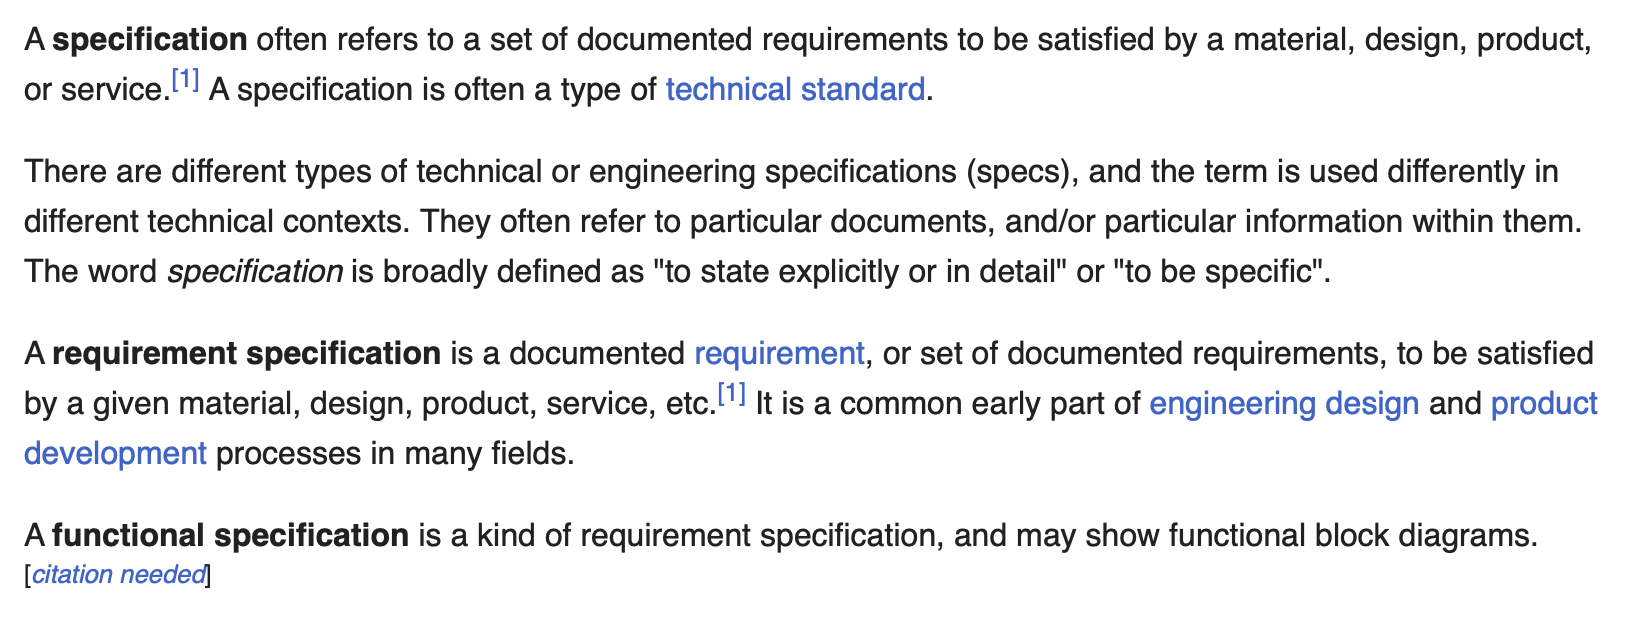
\includegraphics[scale=0.52]{Images/specs}
\end{frame}


\begin{frame}{Lesson 2}{}
\Huge{What is a software specification?}
\includegraphics[scale=0.52]{Images/sfwspecs}
\end{frame}


\begin{frame}{Lesson 2}{}
\Huge
	A \textbf{Software Specification} is a 
	\alert{written} description of what a system is supposed to do.
\end{frame}


\begin{frame}{Lesson 2}{}
\LARGE
\textbf{Software specification}\\~\\
helps us understand our software. It’s a good idea to understand a
system before building it, so it’s a good idea to write a specification of a program
\alert{before} implementing it.
\end{frame}


\begin{frame}{Lesson 2}{}
\LARGE
\textbf{But how can we write the specification?}\\~\\
\begin{itemize}
    \item English? Finnish? Chinese? Words or sentences
    \item Graphical diagrams? Drawing?
    \item Programmable? Coding?
\end{itemize}

\Large
\textbf But all these are imprecise. How can we be precise? What does it mean to be precise?
\end{frame}


\begin{frame}{Lesson 2}{}
\Huge
	Imprecision can lead to \alert{\textbf{ERRORS!}}
\end{frame}


\begin{frame}{Lesson 2}{}
\LARGE
\textbf{Precise specifications}\\~\\
Its hard to be precise using English or other language. Thats why in science and 
engineering fields precise specifications have adopted basic maths to describe 
the specifications.
\end{frame}



\end{document}

